% Chapter Template

\chapter{Water waves on the half-line} % Main chapter title

\label{Chapter5} 

\section{Non-local formulation on the half-line}
In Chapter \ref{Chapter4}, we use the $\mathcal{H}$ formulation to obtain the expected, well-known results on the whole line. In this chapter, we use the formulation to study a slightly different problem: the water-wave problem on the half-line. To the best of our knowledge, this is the first time this problem is studied from a formal derivation perspective. Physically, the problem is motivated by the presence of a wall or an impenetrable barrier at $x = 0.$ This requires imposing several conditions on both $\eta, \phi$ at $x = 0.$ As such, we consider the problem \eqref{S2:DimWholeLineProblem} on the horizontal domain $x\in[0,\infty),$ along with the boundary conditions listed below:
\begin{align}
\phi_{x} &= 0, &x &=0, \label{HLBC1}\\
\phi_{z}(0,\eta,t) &= \eta_t(0,t), &(x,z) &= (0,\eta), \label{HLBC2}
\end{align}
In particular, \eqref{HLBC1} implies that the fluid does not leak through the barrier at $x=0,$ and \eqref{HLBC2} governs an interaction between the fluid and the surface at $x = 0.$ Our objective is to derive approximate equations analogous to those derived in Chapter 4. While the wave equation is expected, there is no reason to look forward to the KdV equations. Indeed, a literature review reveals that a KdV-like equation has not been derived on the half-line, in the way that we derive the KdV equation on the whole line from the full water-wave problem. Here, we use the $\mathcal{H}$ formulation to derive an asymptotic model on the half-line, highlight the main differences, and discuss the difficulties that arise. 

To begin, the scalar equation \eqref{S3:Hequation} relating $\eta$ and $\mathcal{H}$ remains the same, while the non-local, dimensionless equation \eqref{S3:NDimHbehav} becomes
\begin{equation*}%\label{S5:DimHLRP2}
\int_{0}^{\infty} \cos(kx) \cosh(\mu k(\eta+1)) f(x) + \sin(kx) \sinh(\mu k(\eta+1))\mathcal{H}(\epsilon \eta,D) \{f(x) \} \D x = 0.
\end{equation*} 
It is worth noting that taking the real part of \eqref{S3:NDimHbehav} and restricting integrals to $[0,\infty)$ yields the half-line, non-local equation.

By the same procedure, the first two terms in the expansion of $\mathcal{H}$ operator, \eqref{S4:OpPerturbedH1} and \eqref{S4:OpPerturbedH2}, are given by Fourier cosine and sine transforms (defined in front matter):
\begin{align*}
\mathcal{H}_0(\epsilon\eta, D) \{f(x) \} &=  - \invSFT{ \coth(\mu k) \reallywidehat{f^k_c} }, \\
\mathcal{H}_1(\epsilon\eta, D) \{f(x) \} &= - \invSFT{ \mu k \reallywidehat{\left( \eta f(x) \right)}^k_c + \mu k \coth(\mu k) \reallywidehat{\left( \eta \mathcal{H}_0\{f(x) \} \right)}^k_c }.
\end{align*}
The notable difference from the whole-line is the presence of Fourier cosine and sine transforms, in place of Fourier transform. 

We proceed as before in Section \ref{SrfcSec}. Within $\mathcal{O}(\mu^2),$ the scalar equation results into an equivalent of \eqref{S3:Eq18}:
\begin{equation}\label{S5:SurfaceElevationHL}
 \eta_{tt} - \eta_{xx} = \mu^2 \left( \frac{1}{3} \eta_{xxxx}  + \partial_x\invSFT{ \CFT{ \partial_t \left( \eta \int^{x}_0\eta_{t} \D x' \right) } } + \frac{1}{2} \partial^2_x\left(\int^{x}_0\eta_{t} \D x' \right)^2\right).
\end{equation}
The difference between the equations on two domains is the presence of the inverse sine transform of the cosine transform. In particular, this term can be shown to be the Hilbert transform (see Theorem 1 in \cite{Sultan3} for the details).

Now, we seek to derive an asymptotic half-line model. Anticipating secularities, as before we introduce the time scales $\tau_0 = t, \tau_1 = \epsilon t$  and expand $\eta = \eta_0 + \epsilon \eta_1.$ Within $\mathcal{O}(\epsilon^0),$ \eqref{S5:SurfaceElevationHL} becomes $\eta_{0\tau_0 \tau_0} - \eta_{0xx} = 0,$ which is the wave equation. The general solution on the half-line is 
\begin{equation}\label{S5:NS}
\begin{aligned} \eta_0(x, \tau_0, \tau_1) = \begin{cases} F_2(x-\tau_0, \tau_1) + G_2(x+\tau_0, \tau_1) & x\geq \tau_0 \\ F_1(\tau_0-x, \tau_1) + G_1(x+\tau_0, \tau_1) & x < \tau_0 \end{cases}, \end{aligned}
\end{equation}
where $F_i$ and $G_i,$ for $i = 1, 2$ are some general functions. We emphasise that even though $F_1$ and $F_2$ are both left-going waves, they have different domains, and hence are different functions. Similarly, $G_1$ and $G_2$ are different functions, though they are both right-going waves. Finally, that $\eta_0$ is piecewise is the direct consequence of the boundary condition at $x=0.$

As before, initial conditions reveal the dependence of $F_i, G_i, i = 1,2$ on a time scale $\tau_0$ but the dependence on $\tau_1$ is unknown. Following the same procedure as in Section \ref{wKdV}, from \eqref{S5:SurfaceElevationHL} we obtain two half-line versions of \eqref{S3:Eq19}, one valid on $x\geq \tau_0$ and another valid on $x < \tau_0.$ Since the Hilbert-like transform requires additional care, derivations of approximate equations become complicated and are omitted for brevity. 

Removal of secular terms on the two domains yields a system of 4 equations in four unknowns $F_1, F_2, G_1, G_2.$ For $\xi < 0,$ we have
\begin{subequations}\label{S5:HLSystem}
\begin{equation}\label{S5:HLSystem1}
\begin{aligned}
&2 \partial_{\tau_1}F_1 + \frac{1}{3} \partial_\xi^3 F_1 + (F_1-A)\partial_\xi F_1 \\
&+ \frac{1}{\pi} \bigg(\int^0_{-\tau_0} (2 F_1  - A)\partial_{\xi'} F_1\frac{1}{\xi -\xi'} \D \xi' +  \int^{\infty}_{0} (2 F_2 - (A+B))\partial_{\xi'} F_2 \frac{1}{\xi -\xi'} \D \xi'\bigg) = 0, \\
- &2 \partial_{\tau_1} G_1 +  \frac{1}{3} \partial_\zeta^3 G_1 + (G_1+A) \partial_{\zeta} G_1 \\
&+  \frac{1}{\pi} \bigg( \int^{2\tau_0}_{\tau_0} (2 G_1 + A) \partial_{\zeta'} G_1 \frac{1}{\zeta -\zeta'} \D \zeta' + \int^{\infty}_{2\tau_0} (2 G_2+(A+B)) \partial_{\zeta'} G_2 \frac{1}{\zeta -\zeta'} \D \zeta' \bigg) = 0. \\
\end{aligned}
\end{equation} 
For $\xi \geq 0,$ we have
\begin{equation}\label{S5:HLSystem2}
\begin{aligned}
&2 \partial_{\tau_1}F_2 + \frac{1}{3} \partial_\xi^3 F_2 + (F_2-A-B)\partial_\xi F_2 \\
&+ \frac{1}{\pi}  \bigg( \int^0_{-\tau_0} (2 F_1 -A)\partial_{\xi'}F_1\frac{1}{\xi -\xi'} \D \xi' + \int^{\infty}_{0} (2 F_2 -  (A+B))\partial_{\xi'} F_2 \frac{1}{\xi -\xi'} \D \xi'  \bigg) &= 0, \\
-&2 \partial_{\tau_1} G_2 +  \frac{1}{3} \partial_\zeta^3 G_2 + (G_2+ A +B)\partial_{\zeta} G_2 \\
&+ \frac{1}{\pi}  \bigg( \int^{2\tau_0}_{\tau_0} (2 G_1 +A)\partial_{\zeta'} G_1 \frac{1}{\zeta -\zeta'} \D \zeta'  + \int^{\infty}_{2\tau_0} (2 G_2+A+B) \partial_{\zeta'} G_2 \frac{1}{\zeta -\zeta'} \D \zeta' \bigg) &= 0,
\end{aligned}
\end{equation}
\end{subequations}
where $A = F_1(\tau_0)  - G_1(\tau_0),$ and $B = F_2(0) - F_1(0)  +  G_1(2\tau_0) - G_2(2\tau_0).$ Roughly speaking, $A$ comes from nonlocal terms evaluated at $x = 0$ and $B$ arises from nonlocal terms evaluated at $x = \tau_0.$

That the approximate equations are more complicated is expected. Each equation of \eqref{S5:HLSystem} is only slightly similar to KdV: the time derivative is preserved but dispersive and nonlinear terms are different. Note that $F_2$ is defined on $x - t \geq 0$ and $F_1$ is defined on $x - t < 0.$ As such, an $(xt)$-diagram has two regions divided by $x = t$ (see Figure \ref{fig:xtplot}). Physically, the left-going wave $F_1$ is reflected by the barrier at $x = 0,$ inducing certain dynamics on the surface $\eta$ in the \textit{interaction} region $x-t <0.$ A priori, these dynamics are unknown; understanding dynamics in this region is part of the problem. Interestingly, note that if $A = B = 0,$ then dispersion is preserved and a part of nonlinearity is affected by the Hilbert transform.

\begin{figure}[h]
\captionsetup{width=\textwidth}
\centering
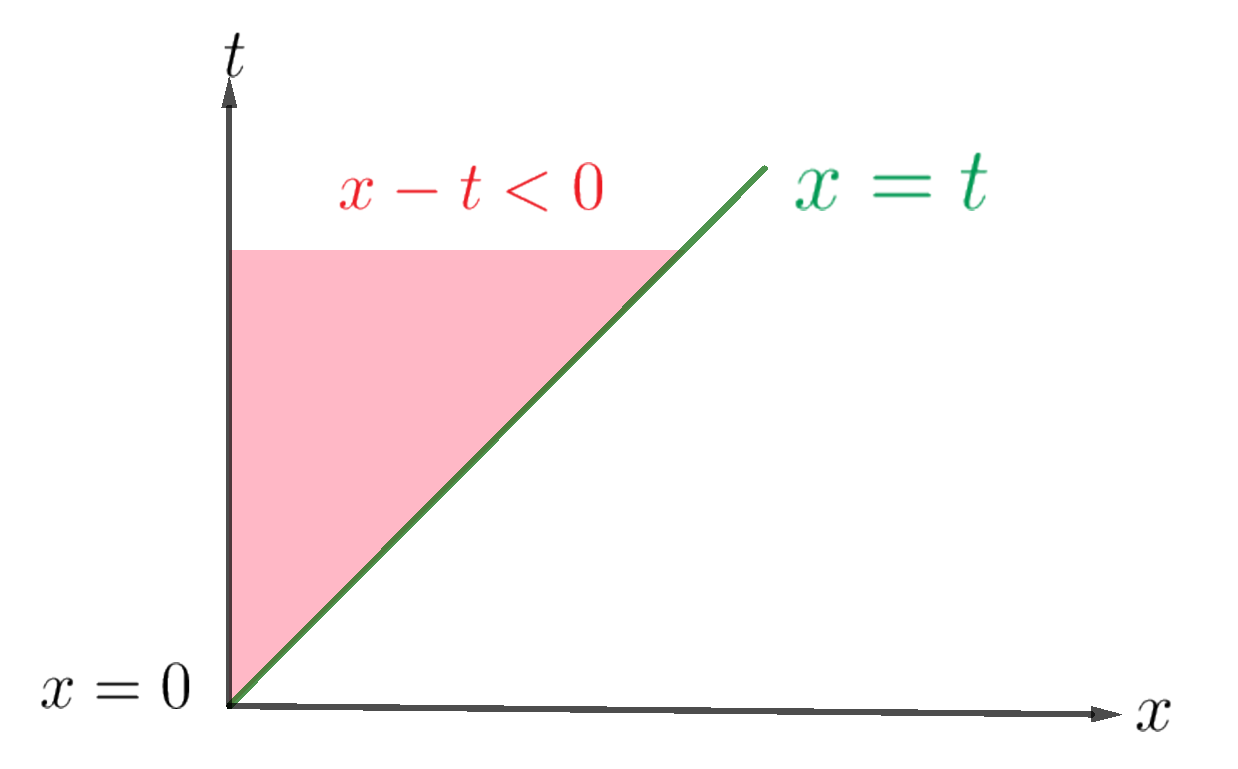
\includegraphics[width=0.6\linewidth]{figures/xtplot.pdf}
\caption{The interaction region in red, for the half-line water-wave problem.}
\label{fig:xtplot}
\end{figure}

A careful look at \eqref{S5:HLSystem} reveals that unlike the whole line case, approximate equations are still dependent on the time scale $\tau_0.$ This is an issue, as the purpose behind  multiple time scales is to separate the dependence on different time scales. As of now, it is not clear why this issue appears. One possible reason is that the linear time scales $\tau_0 = t, \tau_1 = \epsilon t$ should be replaced with different time scales to obtain complete separation.

In sum, although we do not obtain approximate equations on the half-line, we see the utility of the $\mathcal{H}$ formulation in aiding to understand the physical and mathematical difficulties of the half-line problem. This should not be taken for granted. For example, asymptotic expansions via the velocity potential formulation lead to 4 decoupled KdV equations for $F_i, G_i, i =1, 2$, which does not agree with the system \eqref{S5:HLSystem} (see \cite{Sultan1}). As such, the $\mathcal{H}$ formulation shows that the half-line problem has several subtleties,  not readily seen via other formulations. 

\section{Concluding remarks}

In this project, we examine the shallow water limit of the one dimensional water-wave problem, using the $\mathcal{H}$ formulation as developed in \cite{OV2013}. This capstone project presents two contributions to the field of nonlinear waves and raises two future directions. 

First, using the $\mathcal{H}$ formulation, we show that water-wave problem reduces to the well-known KdV model. Since we can easily estimate the order of the normal-to-tangential $\mathcal{H}$ operator, the derivation is especially straightforward. One subtle issue that we sidestep is the \textit{equivalence} of the $\mathcal{H}$ formulation to the velocity potential formulation \eqref{S2:DimWholeLineProblem}. While it is clear that solutions of \eqref{S2:DimWholeLineProblem} solve the $\mathcal{H}$ formulation, the opposite is not so obvious. Without such equivalence, we cannot investigate another aspect of the problem, namely the stability of travelling wave solutions. Therefore, we would like to prove the equivalence, to establish the relevance of the $\mathcal{H}$ formulation with regards to other aspects of the water-wave problem.

Second, we demonstrate the utility of the $\mathcal{H}$ formulation by analysing the water-wave problem on the half-line. Although we do not obtain a KdV-like model, \eqref{S5:SurfaceElevationHL} presents the distinct features and the associated difficulties of the problem. Furthermore, \eqref{S5:SurfaceElevationHL} itself is a new, formally derived asymptotic model for bidirectional waves on the half-line. To the best of our knowledge, the decoupled asymptotic model on the half-line has yet to be derived, and achieving this task may provide additional insights into the physics and mathematics of the problem. In particular, the asymptotic model might describe the surface dynamics in the interaction region $x-t <0.$ This direction is the focus of ongoing research.